\chapter{Proposed Approach}

%This chapter present a general description of the proposal.
The project addresses the high requirements in bit rate for representing HD video content specifically for transmission through the cloud. For solving this problem, is proposed to use the techniques of compressive sensing in video coding and the elements of fog computing. The proposed approach have two main components:
\begin{description}
\item[encoder:] this component involves the calculus of sparse vectors for representing the video frames.
\item[decoder:] this component involves the reconstruction of the video frames based on the sparse vectors generate by the encoder.
\end{description}

The first step is the training of the dictionary. This dictionary is constructed based on a learning algorithm and can be trained in real-time or can be trained offline and preloaded. Generally, the algorithms trained using patches of video frames; depending on the algorithm and needs, the patches are taken from the video original to encode or from predefined video samples. This consideration should be evaluated in the initial part of the project. \\

Once the dictionary is built, the sparse representation for frames of video sequence are calculated. Each video frame is transmitted to the encoder and in the encoder are constructed the sparse $\boldsymbol{\alpha}$ vector for sparse representation. For this, the values of luminance of the video frame are vectorized in $\boldsymbol{y}$ and, with dictionary $\boldsymbol{D}$, is calculated the vector $\boldsymbol{\alpha}$ that represent $\boldsymbol{y}$ through a lineal combination. The main idea of sparse representation is that vector $\boldsymbol{\alpha}$ contains many zero values as is presented in the Fig. \ref{fig:proposed_sparse}. \\

\begin{figure}[!h]
\centering
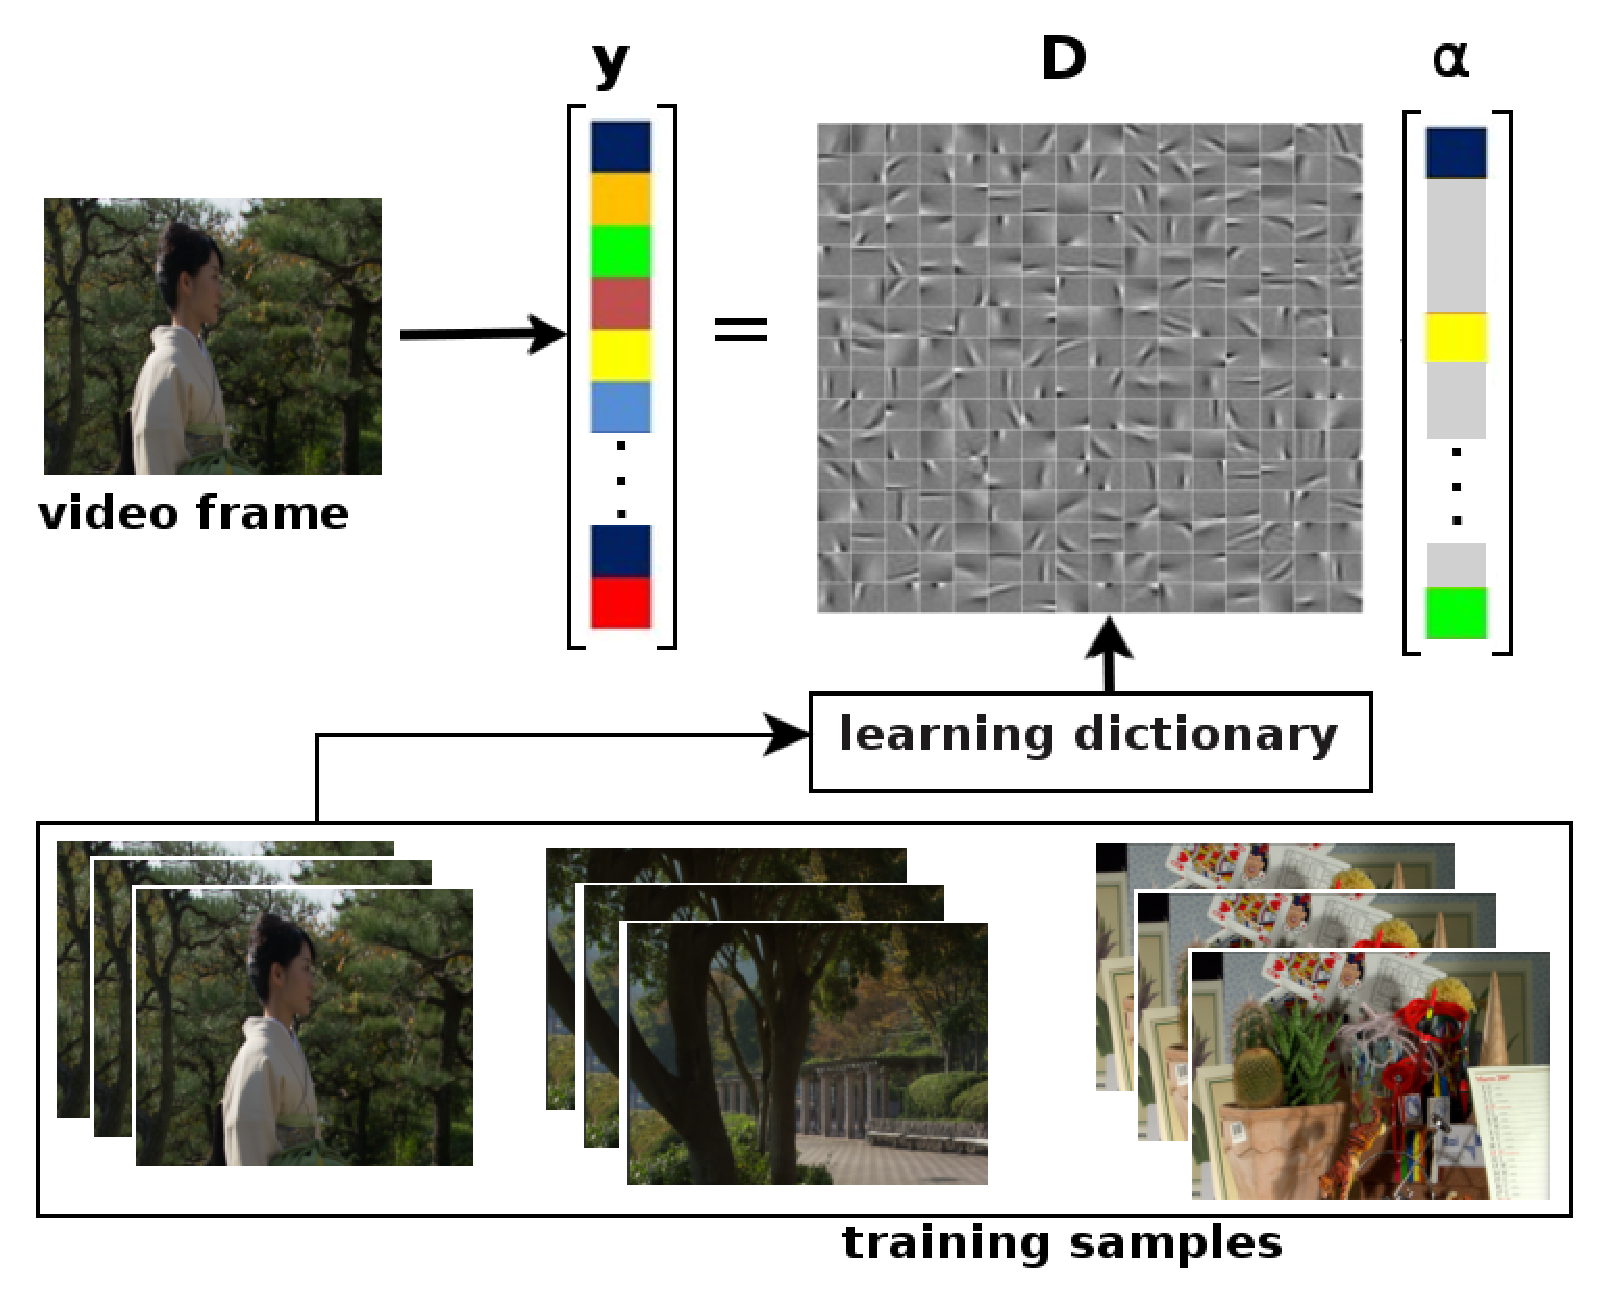
\includegraphics[width=0.45\textwidth]{images/proposed_sparse.eps}
\caption{Sparse representation for video frame}
\label{fig:proposed_sparse}
\end{figure}

The calculated sparse $\alpha$ vector and the dictionary are compressed for reducing the bit for transferring easily. All encoder process is performed in the fog network. In this case, the encoder is implemented using the virtualisation technologies in the edge of the network, with the purpose of reduce the latency compared to the cloud. \\

The information is transferred to the decoder that receives the compressed dictionary $\boldsymbol{D}$ and the sparse vectors $\boldsymbol{\alpha}$,  for decompressing and reconstructing the video frames $\boldsymbol{y}$. The decoder is localised in the end-user.

For the evaluation of coding efficiency are used the Peak Signal-Noise Ratio (PSNR) to evaluated the video quality and the Kbits per second to evaluate the bit rate.
 

